\documentclass[12pt]{article}
\usepackage[a4paper, total={7.5in, 11in}]{geometry}
\usepackage{array}
\usepackage{graphicx, subfig, wrapfig, fancyhdr, lastpage, multicol ,color,arydshln,makecell}

\newcommand\headerMe[2]{\noindent{}#1\hfill#2}
\usepackage[mathscr]{euscript}
\usepackage{tabularray}

\setlength{\columnseprule}{1pt}
\def\columnseprulecolor{\color{blue}}


\pagestyle{fancy}
\fancyhf{}

\cfoot{ \vspace{-0.8cm}\em{Page \thepage \hspace{1pt} / \pageref{LastPage}}}
\begin{document}

\headerMe{Royaume du Maroc}{année scolaire \emph{2022-2023}}\\
\headerMe{Ministère de l'Éducation nationale, }{  Professeur :\emph{Zakaria Haouzan}}\\
\headerMe{du Préscolaire et des Sports}{Établissement : \emph{Lycée SKHOR qualifiant}}\\
%\vspace{-1cm}
\begin{center}
Devoir Surveillé  N°4 - S1 \\
    2ème année baccalauréat Sciences physiques\\
Durée 3h00
\\
    \vspace{.2cm}
\hrulefill
\Large{Chimie 7pts - 63min}
\hrulefill\\

    %\emph{Les deux parties sont indépendantes}
\end{center}
%end Headerss------------------------
%__________________Chimie ______________________-
%%%%%%%+_+_+_+_+_+_+_+_+_Partie1

 \section*{Partie 1 : Etude du vinaigre commercial \dotfill(07pts)-63min }
%\begin{wrapfigure}{r}{0.16\textwidth}
	%\vspace{-1.2cm}
%%\begin{center}
  %%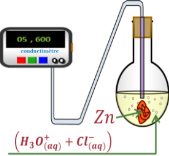
\includegraphics[width=0.16\textwidth]{./img/chimie01.png}
%%\end{center}
%\end{wrapfigure}


%\begin{wrapfigure}[12]{r}{0.38\textwidth}
	%\vspace{-2.4cm}
%\begin{center}
  %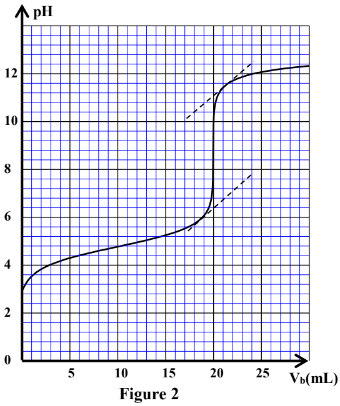
\includegraphics[width=0.38\textwidth]{./img/img00.png}
%\end{center}
%\end{wrapfigure}

 \emph{Le vinaigre est une solution aqueuse d’acide éthanoïque ($CH_3COOH$), il est
caractérisé par son degré d’acidité (X°) qui représente la masse (en gramme)
d’acide éthanoïque contenue dans 100 g de solution.}

\textbf{Données : }
\begin{itemize}
	\item Toutes les mesures ont été faites à 25°C .
	\item La masse volumique du vinaigre : $\rho = 1 g/mL$.
	\item La masse molaire de l’acide éthanoïque : $M(CH_3COOH) = 60 g.mol^{-1}$.
	\item La conductivité molaire ionique de l’ion $H_3O^+$ : $\lambda_{(H_3O^+)} = 3,49.10^{-2}S.m^2.mol^{-1}$.
	\item La conductivité molaire ionique de l’ion $CH_3COO^-$ : $\lambda_{(CH_3COO^-)} = 4,09.10^{-3}S.m^2.mol^{-1}$.
	\item Rappel : La conductivité $\sigma$ s’écrit en fonction des concentrations molaires effectives
		des ions $X_i$ et de leurs conductivités molaires ioniques $\lambda_i$ comme suit : $\sigma = \sum \lambda_i[X_i]$
\end{itemize}

\hspace{-1cm} \textbf{1. Etude de la dissolution de l’acide éthanoïque dans l’eau. \dotfill}

On dispose de deux solutions $(S_1)$ et $(S_2)$ d’acide éthanoïque.
\begin{itemize}
	\item La conductivité de la solution $(S_1)$ de concentration molaire $C_1 = 5.10^{-2} mol.L^{-1}$ est $\sigma_1 = 3,5.10^{-2}S.m^{-1}$.
	\item La conductivité de la solution $(S_2)$ de concentration molaire $C_2 = 5.10^{-3} mol.L^{-1}$ est $\sigma_2 = 1,1.10^{-2}
		S.m^{-1}$.
\end{itemize}

On considère que la dissolution de l’acide éthanoïque dans l’eau est limitée. 

\begin{tabular}{c | c}
		0,75 & \makecell[l]{\textbf{1.1. }Ecrire l’équation modélisant la dissolution de l’acide éthanoïque dans
l’eau.}\\

			0,75 & \makecell[l]{\textbf{1.2. }Trouver l’expression de la concentration molaire effective $[H_3O^+]_{(eq)}$ des
ions oxoniums à \\l’équilibre en fonction de $\sigma$,$\lambda_{(H_3O^+)}$ et $\lambda_{(CH_3COO^-)}$.  }\\

			0,5 & \makecell[l]{\textbf{1.3. }Calculer $[H_3O^+]_{eq}$ dans chacune des solutions $(S_1)$ et $(S_2)$.}\\
			1 & \makecell[l]{\textbf{1.4. }Déterminer les taux d’avancement final $\tau_1$ et $\tau_2$ de la réaction de l’acide
éthanoïque avec \\l’eau dans chacune des solutions $(S_1$) et $(S_2)$. Déduire
l’influence de la concentration initiale de \\la solution sur le taux
d’avancement final. }\\

				1 & \makecell[l]{\textbf{1.5. }Déterminer la constante d’équilibre de la réaction de l’acide éthanoïque
avec l’eau pour \\chacune des solutions $(S_1)$ et ($S_2)$. Conclure. }\\

	
\end{tabular}
			
						\hspace{-1cm}\textbf{2. Vérification du degré d’acidité du vinaigre commercial\dotfill}
On extrait un échantillon de vinaigre commetcial, de volume $V_0 = 1 mL$, de
concentration molaire $C_0$ et portant l’indication (7°), on y ajoute de l’eau distillée
pour préparer une solution (S) de concentration molaire $C_S$ et de volume $V_S=100 mL$.
On neutralise un échantillon de volume VA= 20 mL de la solution (S) à l’aide d’une
solution aqueuse $(S_B)$ d’hydroxyde de sodium  $ (Na^+_{eq} + OH^-_{eq} )$ de concentration molaire $C_B = 1,5.10^{-2} mol.L^{-1}$.L’équivalence est obtenue lorsque le volume vérsé de la solution $(S_B)$ est :
$V_{BE} = 15,7 mL$.
						
\begin{tabular}{c|l}
	0,75  & \makecell[l]{ \textbf{2.1. }Ecrire l’équation modélisant la réaction ayant lieu au cours du dosage.}\\

	0,75	 & \makecell[l]{\textbf{2.2. }Calculer la valeur de $C_S.$  }\\

	1,5 & \makecell[l]{\textbf{2.3. }Déterminer le degré d’acidité du vinaigre étudié. Le résultat obtenu est-il\\
en accord avec l’indication inscrite sur le vinaigre commercial ou non ?}\\

\end{tabular}

%\begin{center}
%\begin{tabular}{ |c| c|}
%\hline
%\textbf{Couple acide/base} &\textbf{ Valeur de $pK_A$}\\\hline
	%$HCOOH / HCOO^-$  & 3,75 \\\hline
	%$C_6H_5COOH/C_6H_5COO^-$ &4,2\\\hline
	%$CH_3COOH/CH_3COO^-$&  4,75 \\\hline
	%$CH_3-CH_2-COOH/CH_3-CH_2-COO^-$ &4,9 \\\hline

%\end{tabular}
%\end{center}

%\begin{tabular}{c|l}
	%0,5 & \makecell[l]{\textbf{3. }Déterminer le volume
	%$V_{b1}$ de la solution $S_b$ versée, au cours du dosage, pour que: $\frac{[AH]}{[A^-]} = 2,24$ . }\\
%\end{tabular}

%\hrulefill
%\Large{Physique 13pts/78min}
%\hrulefill\\
\newpage
\begin{center}
    %\vspace{.60cm}
\hrulefill
\Large{Physique 13pts - 75min}
\hrulefill\\
    %\emph{Les  parties sont indépendantes}
\end{center}

%\vspace{-1cm}
\section*{Exercice 1 – Les ondes – Mesure du diamètre d’un fil \dotfill(03pts)}

%\begin{wrapfigure}[9]{r}{0.25\textwidth}
  %\begin{center}
	  %\vspace{-1cm}
	%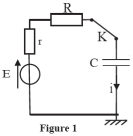
\includegraphics[width=0.19\textwidth]{./img/img01.png}
	%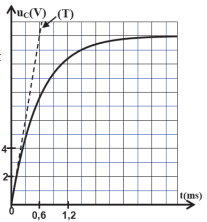
\includegraphics[width=0.25\textwidth]{./img/img02.png}
  %\end{center}
%\end{wrapfigure}
\emph{Les rayons lasers sont utilisés dans plusieurs domaines, grâce à leurs propriétés
optiques et énergétiques. Parmi ces utilisations, on cite la détermination des
dimensions microscopiques de quelques corps.}

Pour mesurer le diamètre d’un fil fin, on réalise les deux expériences suivantes : 


\hspace{-1cm}\textbf{1- Expérience 1 :  \dotfill}

On éclaire une plaque (P) contenant une fente de largeur $a_1$, avec une lumière
monochromatique de longueur d’onde $\lambda$ issue d’une source laser. On observe sur un
écran E placé à une distance $D = 1,6 m$ de la fente (figure 1), un ensemble de taches
lumineuses dont la largeur de la tache centrale est $L_1 = 4,8 cm$ (figure 2).

\begin{center}
	  \vspace{-1cm}
	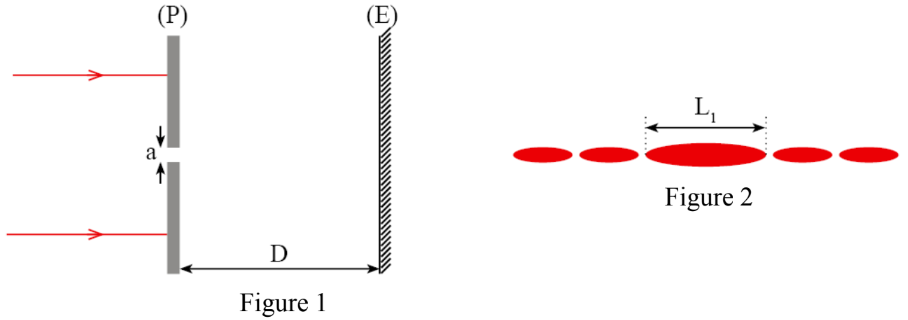
\includegraphics[width=0.6\textwidth]{./img/LesOndes01.png}
	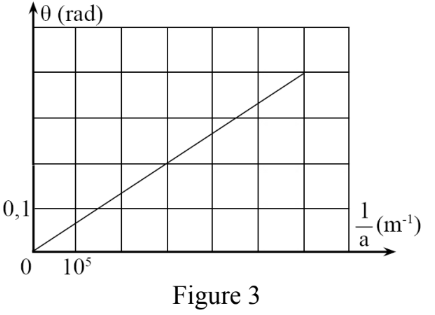
\includegraphics[width=0.3\textwidth]{./img/LesOndes02.png}
  \end{center}

\begin{tabular}{c|l}

	
	0,5 & \makecell[l]{\textbf{1.1. }Recopier la figure 1, et représenter les rayons lumineux après la traversée
de la fente. \\Donner le nom du phénomène illustré par la figure 2 sur
l’écran E. }\\

	0,25 & \makecell[l]{\textbf{1.2. }Quel est la condition que doit satisfaire la largeur a de la fente pour que se
\\phénomène se produisse ? }\\
	
	0,25 & \makecell[l]{\textbf{1.3. }Ecrire l’expression de l’écart angulaire $\theta$ entre le milieu de la tache centrale
et le milieu \\de la première extinction en fonction de $L_1$ et D. }\\
	
	 & \makecell[l]{\textbf{1.4. } La courge de la figure 3, représente les variations de $\theta$ en fonction
	de $\frac{1}{a}$.}\\
	
	0,5 & \makecell[l]{\textbf{1.4.a. }Comment varie la largeur de la frange centrale avec a ? }\\
	1   & \makecell[l]{\textbf{1.4.b. }Déterminer graphiquement $\lambda$ et calculer $a_1$.  }\\
	\end{tabular}

\hspace{-1cm}\textbf{2- Expérience 2 :  \dotfill(0,5pts)}

	On remplace la plaque (P) par un fil fin
de diamètre d, qu’on fixe à la même
distance D de l’écran. On obtient une
figure semblable à la figure 2, mais dont
la largeur de la tache centrale est
$L_2 = 2,5 cm$. Calculer d.


\section*{Exercice 2 – Transformations nucléaires – Applications dans le domaine médical. \dotfill(02pts)}
\emph{La médecine est l'un des principaux domaines ayant connu plusieurs applications de
la radioactivité. On utilise dans ce domaine plusieurs éléments radioactifs pour
diagnostiquer et traiter quelques maladies. Parmi ces éléments, on trouve le Sodium
$^{24}_{11}Na$ qui permet de suivre la circulation sanguine dans le corps humain.}

\begin{tabular}{c|l}	

	  & \makecell[l]{\textbf{1. }Le nucléide Sodium $^{24}_{11}Na$ se désintègre en Magnésium $^{24}_{12}Mg$ .}\\
	0,5 & \makecell[l]{\textbf{1.1. }Ecrire l’équation de désintégration du Sodium 24 en précisant la nature de
cette \\radioactivité.  }\\
	0,25 & \makecell[l]{\textbf{1.2. }Calculer la constante radioactive $\lambda$ de ce nucléide, sachant que\\ la demi-vie
	du Sodium 24 est : $t_{1/2} = 15 h.$ }\\
	
	 & \makecell[l]{\textbf{2. } A la suite d’un accident de route, une personne a perdu un volume de sang.
Pour \\déterminer ce volume, on injecte à ce blessé, à l’instant $t_0 = 0$, un volume
$V_0 = 5 ml$ d’une \\solution de sodium 24 de concentration molaire
$C_0 = 10^{-3} mol.L^{-1}$. }\\
	0,5 & \makecell[l]{\textbf{2.1. }Calculer $n_1$, la quantité de la matière de sodium 24 qui reste dans le sang du
blessé \\à l’instant $t_1 = 3h$. }\\

		0,25 & \makecell[l]{\textbf{2.2. }Calculer l’activité de cet échantillon à cet instant $t_1$. \\((La constante d’Avogadro $N_A = 6,02.10^{23} mol^{-1}$) }\\
	0,5 & \makecell[l]{\textbf{2.3. }L’analyse d’un volume $V_2 = 2,00 ml$ prélevé du sang du même patient, à
		l’instant $t_1 = 3 h$,\\ a montré qu’il contient $n_2 = 2,1.10^{-9} mol$ de Sodium 24.
Déduire la valeur du volume $V_P$ du \\sang perdu, sachant que le corps
humain contient 5 L de sang, où le Sodium est \\répartit uniformément. }\\
\end{tabular}

\section*{Exercice 3 – Electricité – Utilisation d'un condensateur. \dotfill(03pts)}

\emph{Les condensateurs sont caractérisés par la capacité d’emmagasiner l’énergie
électrique, à fin de la récupérer en cas de besoin. Cette propriété permet d’utiliser
les condensateurs dans différents appareils comme les flashs d’appareils photos.}


\hspace{-1cm}\textbf{Partie 1:  Charge du Condensateur :\dotfill}

On réalise le montage représenté ci-contre et
qui est constitué d’un condensateur de capacité
C, initialement déchargé, monté en série avec
un conducteur ohmique de résistance R et un
interrupteur K.
Le dipôle RC est soumis à un échelon de tension défini comme suit : 

-Pour $t < 0$, $U=0$ , 

-Pour $t\geq 0$ , $U=E=12V$.

\begin{center}
	  \vspace{-1cm}
	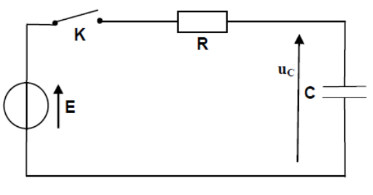
\includegraphics[width=0.3\textwidth]{./img/RC00.png}
	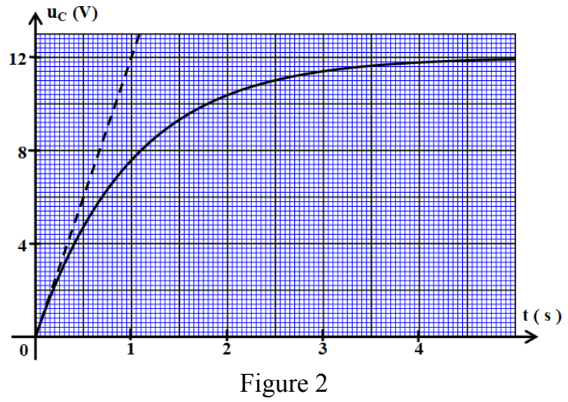
\includegraphics[width=0.4\textwidth]{./img/RC01.png}
  \end{center}

On ferme le circuit à l’instant
$t = 0$ et on visualise, en
utilisant une interface
informatique sur l’écran d’un
ordinateur les variations de la
tension uc aux bornes du
condensateur en fonction du
temps.
Le graphe de la figure 2
représente la courbe $u_c = f(t)$.

\begin{tabular}{c|l}	

	0,5  & \makecell[l]{\textbf{1.1. }Etablir l’équation différentielle vérifiée par la tension $u_c(t)$.}\\
	0,5  & \makecell[l]{\textbf{1.2. }Vérifier que l’expression $u_c(t) = E(1-e^{-\frac{t}{\tau}}),$ est solution de l’équation
différentielle pour \\$t \geq 0$,$\tau$ est la constante de temps. }\\

	 0,5 & \makecell[l]{\textbf{1.3. }Déterminer l’expression de $\tau$, et montrer par analyse dimensionnelle que $\tau$
est homogène à \\un temps un temps. }\\

	  0,5 & \makecell[l]{\textbf{1.4. }Noter graphiquement la valeur de $\tau$, et vérifier que la valeur de la capacité
du condensateur \\est $C = 100 \mu F$.On donne $R=10 K.\Omega$. }\\
	  1 & \makecell[l]{\textbf{1.5. }Calculer l’énergie électrique emmagasinée par le condensateur en régime
permanent. }\\
\end{tabular}



\section*{Exercice 4 – Electricité – Principe de production d’une étincelle \dotfill(5pts)}
La production d’étincelles dans le moteur d’une voiture nécessite deux circuits :
\begin{itemize}
	\item Circuit primaire constitué d’une bobine de coefficient d’inductance L et de
résistance r alimentée par la batterie de la voiture

\item Circuit secondaire constitué d’une autre bobine et une bougie d’allumage.
\end{itemize}
L’ouverture du circuit primaire provoque une étincelle qui jaillit entre les bornes de
bougie d’allumage et amorce la combustion du mélange air-essence. Cette étincelle
apparait lorsque la tension entre les bornes de la bougie d’allumage dépasse la
valeur U = 10000 V.

\begin{center}
	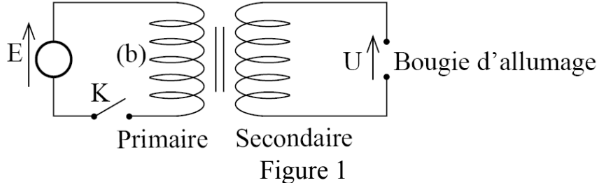
\includegraphics[width=0.4\textwidth]{./img/RL00.png}
	  \vspace{-0.5cm}
  \end{center}


On modélise le système d’allumage dans le moteur d’une voiture par le montage
représenté dans la figure 1.

\hspace{-1cm}\textbf{Partie I : Etablissement du courant dans le circuit primaire :  \dotfill}

On modélise le circuit primaire par le montage de la figure 2, où :

\begin{itemize}
	\item G : Batterie de voiture assimilée à un générateur
idéal de tension continue de f.é.m E = 12 V.
\item (b) : Bobine d’inductance L et de résistance
interne $r = 1,5 \Omega$.
\item D : Un conducteur ohmique équivalent au reste
du circuit de résistance $R = 4,5 \Omega$ , K : Interrupteur

\end{itemize}


\begin{center}
	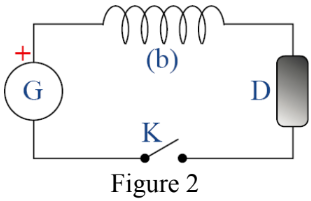
\includegraphics[width=0.3\textwidth]{./img/RL01.png}
	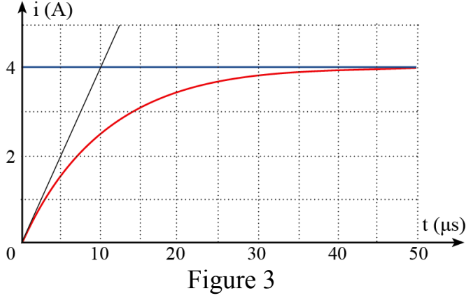
\includegraphics[width=0.3\textwidth]{./img/RL02.png}
	  \vspace{-0.5cm}
  \end{center}



\hspace{-0.8cm}
\begin{tabular}{c|l}	

	 & \makecell[l]{\textbf{1. }On ferme l’interrupteur K à l’instant t = 0, le circuit est alors traversé par un
courant électrique i(t).}\\
	0,5 & \makecell[l]{\textbf{1.1. }Recopier le circuit de la figure 2 et représenter dessus les tensions en
convension récepteur. }\\
	1 & \makecell[l]{\textbf{1.2. }Montrer que l’équation differentielle vérifiée par le courant i(t) s’écrit sous
	la forme: $\frac{di}{dt}+\frac{i}{\tau} = A$, \\en précisant les expression de $\tau$ et A.}\\
	
	0,5 & \makecell[l]{\textbf{1.3. }Montrer par analyse
dimensionnelle que la
constante $\tau$ est homogène à
un temps. }\\
	 & \makecell[l]{\textbf{1.4 }La courbe de la figure 3
représente les variation de
l’intensité du courant en
fonction du temps.}\\

	0,5 & \makecell[l]{\textbf{1.4.1 }Déterminer graphiquement la valeur de la constante de temps $\tau$ et
celle l’intensité $I_0$ du courant \\en régime permanent. }\\
	0,5 & \makecell[l]{\textbf{1.4.2 }En déduire la valeur du coefficient d’inductance L de la bobine (b).}\\
\end{tabular}


\hspace{-1cm}\textbf{Partie II : Annulation du courant dans le circuit primaire : \dotfill}
On ouvre le circuit primaire à un instant considéré comme nouvelle origine des
temps t = 0, l’intensité du courant i(t) traversant le circuit diminue alors, et
apparait une étincelle entre les bornes de la bougie d’allumage dans le circuit
secondaire.

\begin{center}
	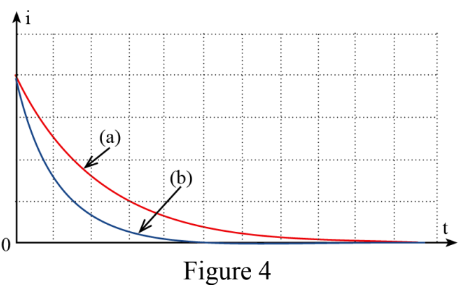
\includegraphics[width=0.3\textwidth]{./img/RL03.png}
	  \vspace{-0.5cm}
  \end{center}



\hspace{-0.8cm}
\begin{tabular}{c|l}	

	0,5 & \makecell[l]{\textbf{2.1. }Préciser entre les deux propositions suivantes de l’expression de i(t), celle qui correspond à \\cet état. Justifier. $i(t) = B(1-e^{-\frac{t}{\tau}})$  , $i(t) = Be^{-\frac{t}{\tau}}$, où B est une constante}\\
		1 & \makecell[l]{\textbf{2.2. }Sur la figure 4 sont
représentées les courbes (a)
et (b) traduisant les
variations de i(t) en fonction
\\du temps pour deux
bobines de même résistance r et de coefficients d’autoinduction différents.\\
Sachant que la tension U dans le circuit secondaire est proportionnelle à $\mid \frac{\Delta{i}}{\Delta{t}} \mid$, et que
l’allumage\\ de la bougie est plus efficace, tant que la tension U est plus grande.
Préciser laquelle des deux \\bobines assure le plus efficace allumage.
}\\

\end{tabular}
	%\vspace{0.5cm}
%\textbf{2. Injection locale d’une solution contenant du rhénium 186.
%Le produit injectable se présente sous la forme d’une solution contenue dans un flacon de volume $V_0= 10 mL$ ayant une activité $a_0 = 4.10^9Bq$ à la date $t=0$, c'est-à-dire à la sortie du laboratoire pharmaceutique.}
	%\begin{tabular}{c|l}

		%1 & \makecell[l]{\textbf{2.1 }Déterminer en jours la valeur de demi-vie $t_{1/2}$ du rhénium $_{75}^{186}Re$}\\

		%0,5 & \makecell[l]{\textbf{2.2 }Trouver, à l’instant $t_1 = 4,8jours$, le nombre $N_1$ de noyau de rhénium contenu dans le flacon.}\\

		%0,5 & \makecell[l]{\textbf{3.2 } À l’instant $t_1$ on prélève du flacon de volume $V_0 = 10mL$ une injection de volume V contenant \\$N = 3,65.10^{13}$ noyaux de rhénium 186, on l’injecte à un malade dans l’articulation de l’épaule, \\trouver la valeur de V.}\\
	%\end{tabular}


%\section*{Partie 2 :  Centrale nucléaire \dotfill(9pts)}
%Dans une centrale nucléaire, les noyaux d'uranium $^{235}_{92}U$ subissent la fission sous le choc d'un neutron
%lent. Un des nombreux processus possibles conduit à la formation d'un noyau de lanthane $^{144}_{57}La$ ,d'un noyau de brome $^{88}_{35}Br$ et  de plusieurs neutrons.

%\begin{tabular}{c|l}

 %1& \makecell[l]{\textbf{1. } Définissez l'énergie de liaison d'un noyau.}\\

 %1 & \makecell[l]{\textbf{2. } Donnez l'expression littérale qui permettra son calcul.}\\

 %1 & \makecell[l]{\textbf{3. } Calculez, en MeV, l'énergie de liaison d’un noyau $^{235}_{92}U$.}\\

 %1 & \makecell[l]{\textbf{4. } Calculez l’énergie de liaison par nucléon de ce noyau.}\\

 %1 & \makecell[l]{\textbf{5. } Ecrivez l’équation de la réaction de fission étudiée.}\\

 %1 & \makecell[l]{\textbf{6. } Exprimez l'énergie libérée par la fission d'un noyau $^{235}_{92}U$ en fonction des énergies de liaison par
%\\ nucléon du noyau père et des noyaux fils et calculez la valeur de cette énergie en MeV.}

 %\end{tabular}

%\textbf{7.  Dans le cœur de la centrale, de nombreuses autres réactions de fission du noyau $^{235}_{92}U$ se produisent. La perte de masse est, en moyenne, de 0,200 u par noyau.}


%\begin{tabular}{c|l}

	%1,5 & \makecell[l]{\textbf{7.1. } Calculez, en MeV, l'énergie moyenne libérée par la fission d’un noyau. Ce résultat est-il \\en concordance avec celui de la question 6 ?}\\

	%1,5 &\makecell[l]{\textbf{7.2. }Calculez, en joule, l'énergie moyenne libérée par une mole de noyaux $^{235}_{92}U$ } 

%\end{tabular}

%\textbf{Données :}
%\begin{itemize}
	%\item Célérité de la lumière dans le vide : $c = 2,998 . 10^8 m.s^{-1}$  
	%\item Masse du noyau d’uranium 235 : $m( ^{235}_{92}U) = 235,0134u$ 

	%\item Energies de liaison par nucléon : $E_l/A(^{144}_{57}La) = 8,28MeV/nucl$éon  ; $E_l/A(^{88}_{35}Br)$=$8,56MeV/nucl$éon
	%\item Constante d'Avogadro : $N_A = 6,02.10^{23} mol^{-1}$
	%\item $1u$ = $1,66055.10^{-27}Kg$ et $1eV = 1,602.10^{-19}J$
	%\item Masse d’un proton : $m(^1_1p) = 1,0073u$ ; Masse d’un neutron $m(^1_0n) = 1,0087u$
%\end{itemize}





\end{document}
